%!TEX root = main.tex
\paragraph{Fast multipole method}

The fast multipole method (\fmm) is an algorithm that can reduce the quadratic time and space complexity of such matrix-vector multiplication down to $\mathcal{O}(N)$.
In the context of \fmm, $\{\mathbf{r}_i\}$ and $\{\mathbf{r}_j'\}$ in Equation \ref{eq:nbody_sum} are often referred to as the set of targets and sources respectively, with $\{q_j\}$ representing the source densities (charges).
The goal of \fmm is to efficiently compute the potential at $N$ targets $\{s_i\}$ induced by all $N$ sources and the kernel function $g$.
Following the common notations in the literature, we use $\mathbf{x}_i$ and $\mathbf{y}_j$, instead of $\mathbf{r}_i$ and $\mathbf{r}_j'$, to denote targets and sources respectively in this subsection.

The \fmm algorithm builds upon two fundamental ideas: (1) approximating the far-range interactions between distant clusters of sources and targets using low-rank methods, while computing the near-range interactions exactly, and (2) partitioning the domain using a tree structure to maximize the far-range portion in the computation.

To construct the octree, we first create a cube that encloses all sources/targets and then recursively subdivide the domain until each cube at the finest level only contains a constant number of points.
Figure \ref{fig:near_far_decomp} depicts a 3-level quadtree.
The potentials of targets in node $B$ consist of three contributions: the influence from sources in the near-field of $B$: $\mathcal{N}(B)$, in the interaction list of $B$: $\mathcal{I}(B)$, and in the rest of the domain.
$B$'s near-field includes $B$ and its neighbors, where the interactions are computed exactly.
The remaining domain is in $\mathcal{F}(B)$, $B$'s far-field.
In $\mathcal{F}(B)$, the nodes that are the children of $B$'s parent's neighbors but are not adjacent to $B$ compose $\mathcal{I}(B)$, the interaction list of $B$, whose contributions to $B$ are approximated by low-rank methods.
The contributions from the rest of the far-field are approximated at coarser levels via $B$'s ancestors.

The classic \fmm \cite{greengard1987fast, cheng1999fast} relies on truncated analytical expansions to approximate far-field interactions, whereas its kernel-independent variant \cite{ying2004kernel} uses equivalent densities (charges) instead.
In \kifmm, each node is associated with upward and downward equivalent densities (see Figure \ref{fig:multipole} and \ref{fig:local}), the analog of multipole and local expansions in the analytical \fmm.
The upward equivalent densities $q^{B,u}$ are used to approximate the influence of sources in $B$ on targets in $\mathcal{F}(B)$;
the downward equivalent densities $q^{B,d}$ are used to approximate the influence of sources in $\mathcal{F}(B)$ on sources in $B$.
To find these densities, we match the potential of equivalent densities to the potential of actual sources at the check surfaces:
%
\begin{align}\label{eq:multipole_local}
    \sum_{\mathbf{y}_{j} \in B} g\left(\mathbf{x}_{i}^{B,u}, \mathbf{y}_{j}\right) q_{j} &= \sum_{j} g\left(\mathbf{x}_{i}^{B,u}, \mathbf{y}^{B,u}_{j}\right) q^{B,u}_{j}, \quad \forall i  \nonumber \\
    \sum_{\mathbf{y}_{j} \in \mathcal{F}(B)} g\left(\mathbf{x}_{i}^{B,d}, \mathbf{y}_{j}\right) q_{j} &= \sum_{j} g\left(\mathbf{x}_{i}^{B,d}, \mathbf{y}^{B,d}_{j}\right) q^{B,d}_{j}, \quad \forall i
\end{align}
%
We then solve the linear systems for $\{q^{B,u}_{j}\}$ and $\{q^{B,d}_{j}\}$.
Here, $\mathbf{x}_{i}^{B}$ and $\mathbf{y}_{j}^{B}$ denote the discretization points of the check surface and equivalent surface of $B$ respectively.

The algorithm also defines the following operators:
%
\begin{itemize}
    \item particle-to-multipole (P2M): For a leaf node $B$, compute $B$'s upward equivalent densities, \ie multipole expansion, from the sources in $B$. (Figure \ref{fig:multipole})
    \item multipole-to-multipole (M2M): For a non-leaf node $B$, evaluate $B$'s multipole expansion based on the multipole expansions of all $B$'s children. (Figure \ref{fig:translations} left)
    \item multipole-to-local (M2L): For a node $B$, evaluate $B$'s downward equivalent densities, \ie local expansion, by using the multipole expansions of all nodes in $\mathcal{I}(B)$. (Figure \ref{fig:translations} middle)
    \item local-to-local (L2L): For a non-leaf node $B$, add the contribution of $B$'s local expansion to the local expansions of $B$'s children. (Figure \ref{fig:translations} right)
    \item local-to-particle (L2P): For a leaf node $B$, evaluate $B$'s local expansion at the locations of targets in $B$.
    This step adds all far-field contribution to the potentials of targets in $B$. 
    \item particle-to-particle (P2P): For a leaf node $B$, evaluate the potential induced by all sources in $\mathcal{N}(B)$ directly.
\end{itemize}
%
As indicated by the arrows in Figure \ref{fig:translations}, translation operators in \kifmm share the same procedure: (1) evaluating the potentials on the check surface, and (2) solving the equation arising from matching the potentials for the equivalent densities.

Figure \ref{fig:fmm_sketch} outlines the complete \fmm algorithm.
During the upward pass, we compute P2M at all leaf nodes and perform M2M in post-order tree traversal.
Next, we compute M2L for all nodes.
Finally, we compute L2L in pre-order tree traversal, and perform L2P and P2P at all leaf nodes during the downward pass.

\begin{figure*}
    \begin{subfigure}{\columnwidth}
        \centering
        \subcaption{An example of a 3-level quadtree.}
        \makebox[\textwidth][c]{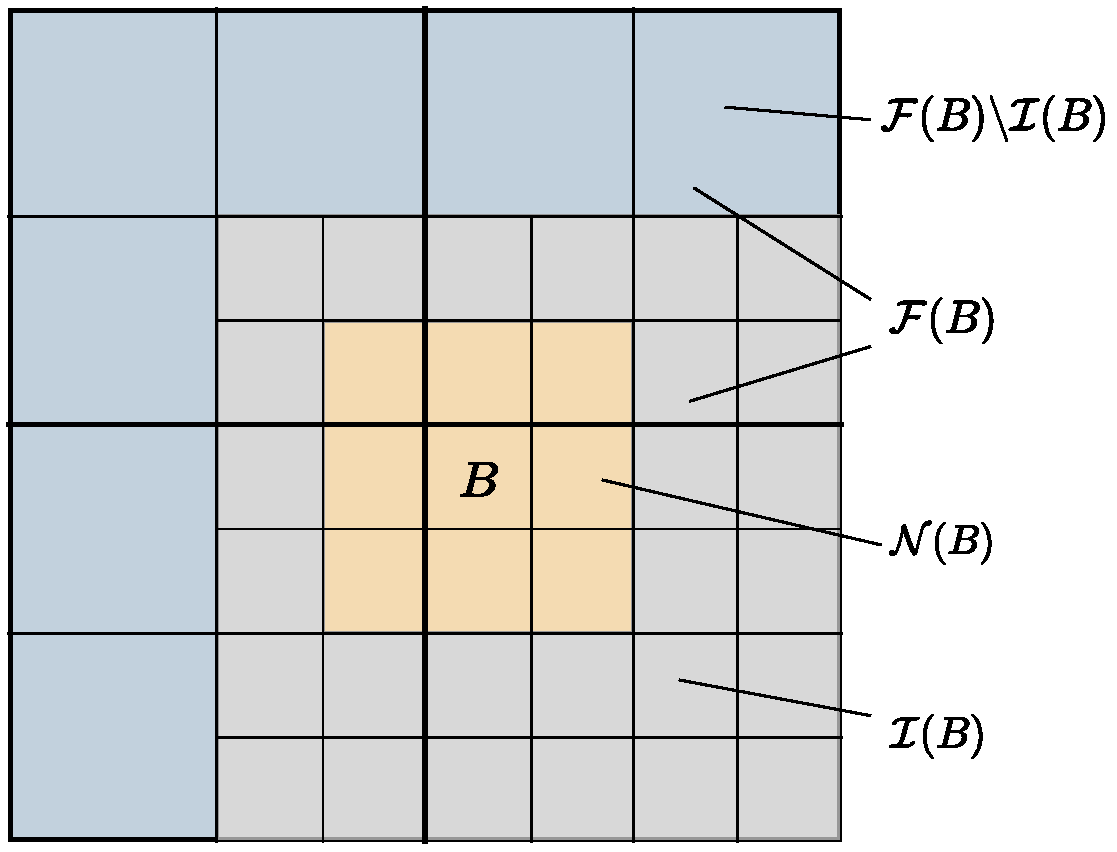
\includegraphics[width=0.7\linewidth]{near_far_decomposition.pdf}}
        \label{fig:near_far_decomp}
    \end{subfigure}
    \begin{subfigure}{\columnwidth}
        \centering
        \subcaption{Sketch of FMM algorithm using a binary tree.}
        \makebox[\textwidth][c]{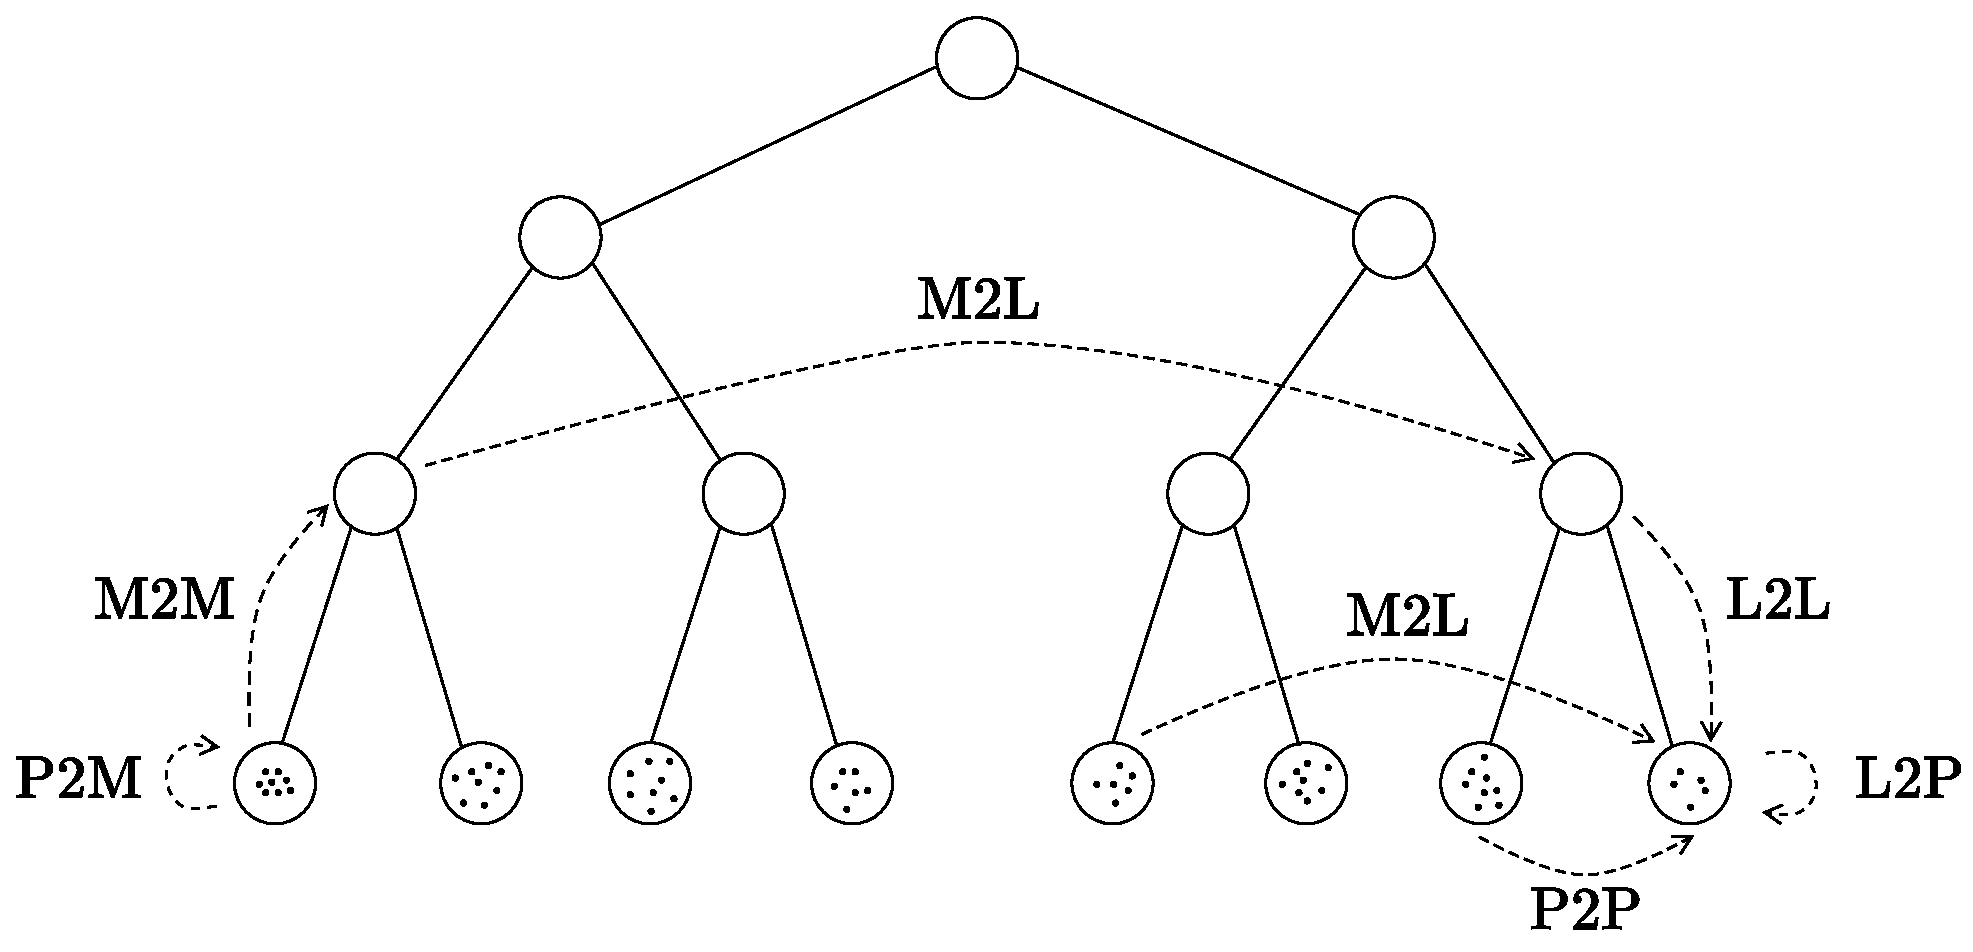
\includegraphics[width=\linewidth]{fmm_sketch.pdf}}
        \label{fig:fmm_sketch}
    \end{subfigure}
    \begin{subfigure}{\columnwidth}
        \centering
        \subcaption{Multipole expansion in \kifmm.}
        \makebox[\textwidth][c]{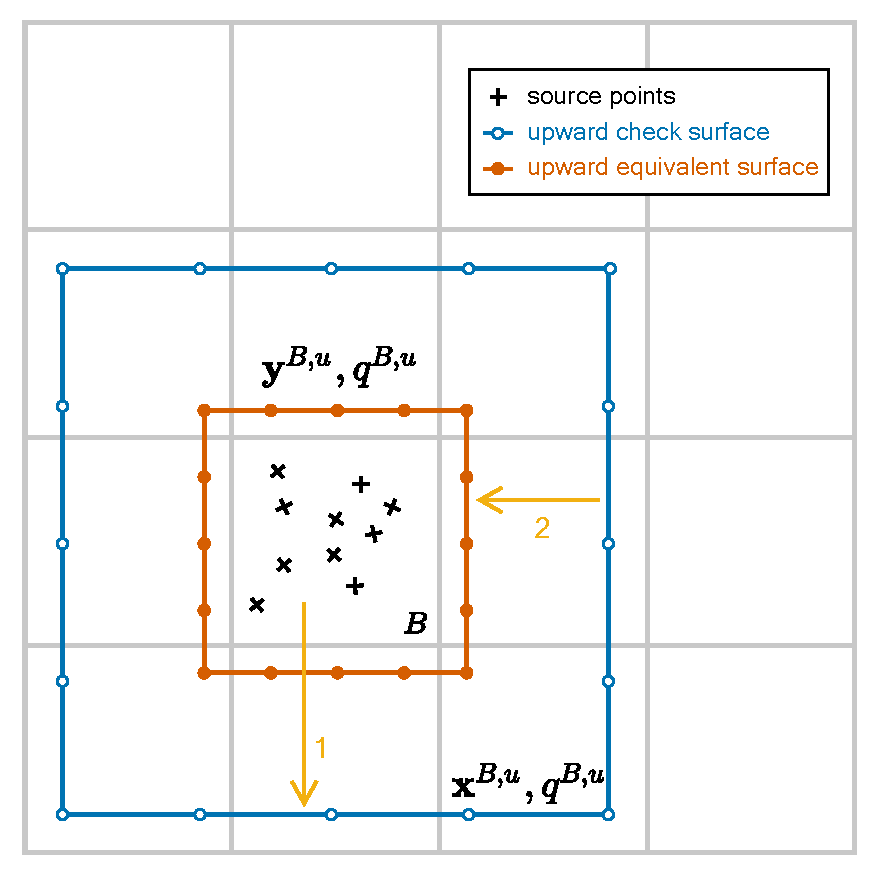
\includegraphics[width=0.7\linewidth]{multipole_expansion.pdf}}
        \label{fig:multipole}
    \end{subfigure}
    \begin{subfigure}{\columnwidth}
        \centering
        \subcaption{Local expansion in \kifmm.}
        \makebox[\textwidth][c]{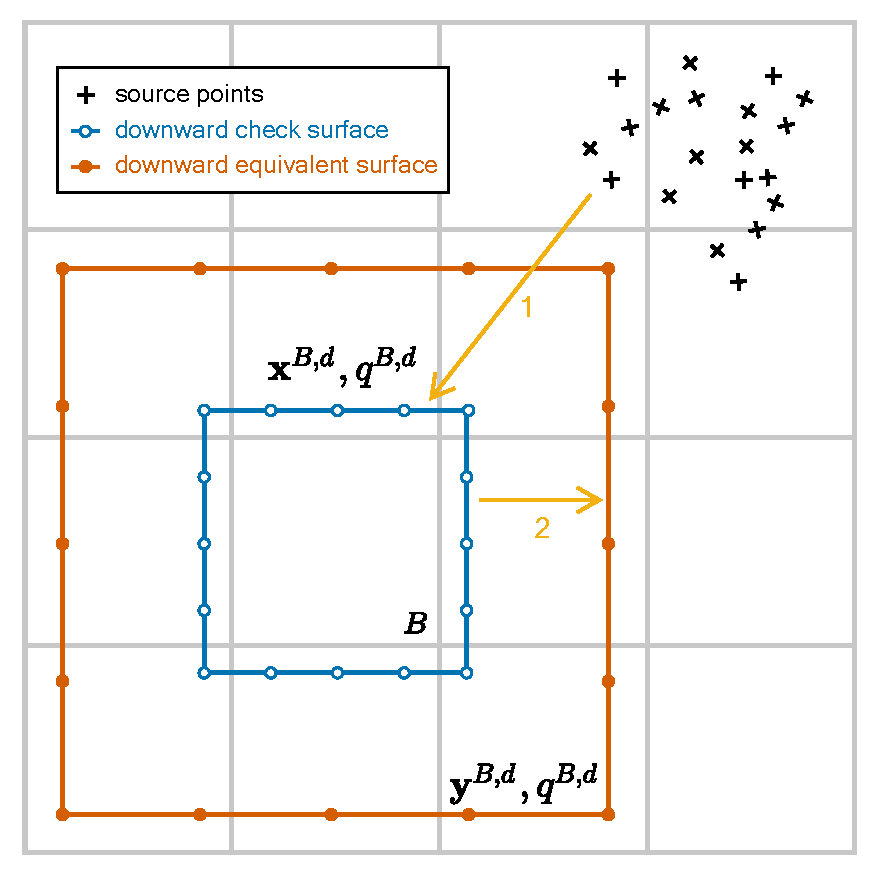
\includegraphics[width=0.7\linewidth]{local_expansion.pdf}}
        \label{fig:local}
    \end{subfigure}
    \begin{subfigure}{\linewidth}
        \centering
        \subcaption{M2M (left), M2L (middle) and L2L (right) operators in \kifmm. Node $C$ is the parent of $B$, and node $A$ is in the interaction list of $B$.}
        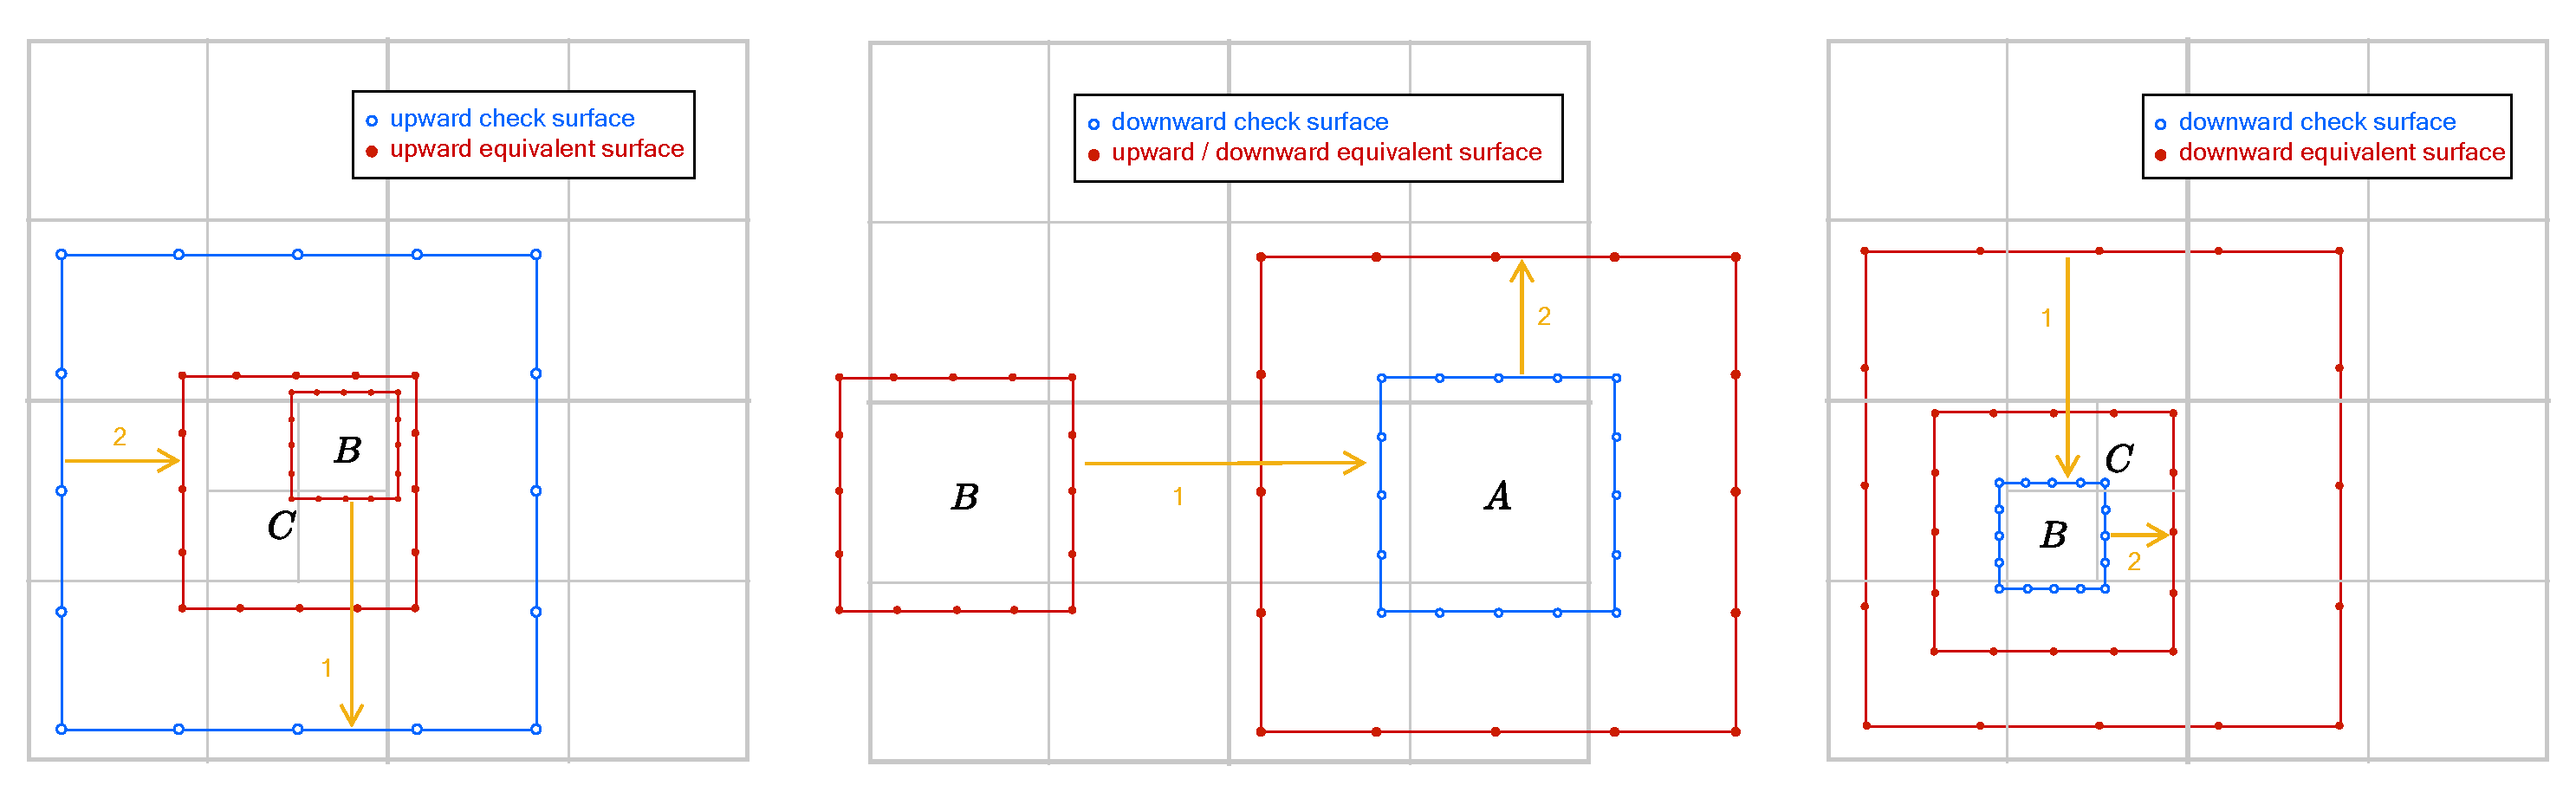
\includegraphics[width=\linewidth]{translations.pdf}
        \label{fig:translations}
    \end{subfigure}
    \caption{Illustrations of the \fmm algorithm.}
\end{figure*}

The original Exafmm \cite{yokota2012tuned,yokota2013fmm} implements the classical \fmm based on dual tree traversal and focuses on low-accuracy optimizations.
Recently, Exafmm received a major update to adopt \kifmm due to its great extensibility.
Its current generation, Exafmm-t, offers highly optimized \kifmm operators, allows pre-computing and caching invariant matrices and more importantly, provides a high-level Python interface to reach a broader audience.